% Options for packages loaded elsewhere
\PassOptionsToPackage{unicode}{hyperref}
\PassOptionsToPackage{hyphens}{url}
\documentclass[
  ignorenonframetext,
]{beamer}
\newif\ifbibliography
\usepackage{pgfpages}
\setbeamertemplate{caption}[numbered]
\setbeamertemplate{caption label separator}{: }
\setbeamercolor{caption name}{fg=normal text.fg}
\beamertemplatenavigationsymbolsempty
% remove section numbering
\setbeamertemplate{part page}{
  \centering
  \begin{beamercolorbox}[sep=16pt,center]{part title}
    \usebeamerfont{part title}\insertpart\par
  \end{beamercolorbox}
}
\setbeamertemplate{section page}{
  \centering
  \begin{beamercolorbox}[sep=12pt,center]{section title}
    \usebeamerfont{section title}\insertsection\par
  \end{beamercolorbox}
}
\setbeamertemplate{subsection page}{
  \centering
  \begin{beamercolorbox}[sep=8pt,center]{subsection title}
    \usebeamerfont{subsection title}\insertsubsection\par
  \end{beamercolorbox}
}
% Prevent slide breaks in the middle of a paragraph
\widowpenalties 1 10000
\raggedbottom
\AtBeginPart{
  \frame{\partpage}
}
\AtBeginSection{
  \ifbibliography
  \else
    \frame{\sectionpage}
  \fi
}
\AtBeginSubsection{
  \frame{\subsectionpage}
}
\usepackage{iftex}
\ifPDFTeX
  \usepackage[T1]{fontenc}
  \usepackage[utf8]{inputenc}
  \usepackage{textcomp} % provide euro and other symbols
\else % if luatex or xetex
  \usepackage{unicode-math} % this also loads fontspec
  \defaultfontfeatures{Scale=MatchLowercase}
  \defaultfontfeatures[\rmfamily]{Ligatures=TeX,Scale=1}
\fi
\usepackage{lmodern}
\ifPDFTeX\else
  % xetex/luatex font selection
\fi
% Use upquote if available, for straight quotes in verbatim environments
\IfFileExists{upquote.sty}{\usepackage{upquote}}{}
\IfFileExists{microtype.sty}{% use microtype if available
  \usepackage[]{microtype}
  \UseMicrotypeSet[protrusion]{basicmath} % disable protrusion for tt fonts
}{}
\makeatletter
\@ifundefined{KOMAClassName}{% if non-KOMA class
  \IfFileExists{parskip.sty}{%
    \usepackage{parskip}
  }{% else
    \setlength{\parindent}{0pt}
    \setlength{\parskip}{6pt plus 2pt minus 1pt}}
}{% if KOMA class
  \KOMAoptions{parskip=half}}
\makeatother
\usepackage{longtable,booktabs,array}
\newcounter{none} % for unnumbered tables
\usepackage{calc} % for calculating minipage widths
\usepackage{caption}
% Make caption package work with longtable
\makeatletter
\def\fnum@table{\tablename~\thetable}
\makeatother
\usepackage{graphicx}
\makeatletter
\newsavebox\pandoc@box
\newcommand*\pandocbounded[1]{% scales image to fit in text height/width
  \sbox\pandoc@box{#1}%
  \Gscale@div\@tempa{\textheight}{\dimexpr\ht\pandoc@box+\dp\pandoc@box\relax}%
  \Gscale@div\@tempb{\linewidth}{\wd\pandoc@box}%
  \ifdim\@tempb\p@<\@tempa\p@\let\@tempa\@tempb\fi% select the smaller of both
  \ifdim\@tempa\p@<\p@\scalebox{\@tempa}{\usebox\pandoc@box}%
  \else\usebox{\pandoc@box}%
  \fi%
}
% Set default figure placement to htbp
\def\fps@figure{htbp}
\makeatother
\setlength{\emergencystretch}{3em} % prevent overfull lines
\providecommand{\tightlist}{%
  \setlength{\itemsep}{0pt}\setlength{\parskip}{0pt}}
% Slide layout defaults for warning-clean scientific decks.
\usepackage{etoolbox}
\IfFileExists{xurl.sty}{\usepackage{xurl}}{}
\IfFileExists{seqsplit.sty}{\usepackage{seqsplit}}{\newcommand{\seqsplit}[1]{#1}}
\protected\def\breakseq#1{\seqsplit{#1}}
\protected\def\breaktt#1{\begingroup\ttfamily\seqsplit{#1}\endgroup}
\setlength{\emergencystretch}{6em}
\tolerance=5000
\hbadness=10000
\hfuzz=1pt
\setlength{\tabcolsep}{2pt}
\AtBeginEnvironment{longtable}{\tiny\renewcommand{\arraystretch}{0.86}\setlength{\tabcolsep}{1pt}}
\AtBeginEnvironment{tabular}{\tiny\renewcommand{\arraystretch}{0.86}\setlength{\tabcolsep}{1pt}}

% Natbib and cross-reference fallbacks — slides don't load natbib
% or cleveref, but combined-PDF manuscript prose may emit these
% commands. The fallback renders citations as a bracketed key list
% and cross-references as detokenized labels so slides don't fail on
% undefined control sequences or raw underscores. \providecommand is
% a no-op if packages load later.
\providecommand{\citep}[1]{[#1]}
\providecommand{\citet}[1]{#1}
\providecommand{\citealp}[1]{#1}
\providecommand{\citeauthor}[1]{#1}
\providecommand{\citeyear}[1]{#1}
\providecommand{\cref}[1]{\texttt{\detokenize{#1}}}
\providecommand{\Cref}[1]{\texttt{\detokenize{#1}}}
\usepackage{bookmark}
\IfFileExists{xurl.sty}{\usepackage{xurl}}{} % add URL line breaks if available
\urlstyle{same}
% fallback for those not using the hyperref driver hyperxmp:
\makeatletter
\@ifundefined{xmpquote}{\newcommand{\xmpquote}[1]{#1}}{}
\makeatother
\hypersetup{
  hidelinks,
  pdfcreator={LaTeX via pandoc}}

\author{\texorpdfstring{}{}}
\date{}

\begin{document}

\section{Results}\label{results}

\begin{frame}[fragile,allowframebreaks]{Results}
\texttt{template/} was evaluated through multi-project pipeline
execution, measuring test coverage, pipeline timing, output integrity,
and steganographic performance across the canonical exemplars under
\texttt{projects/}.
\end{frame}

\begin{frame}[fragile,allowframebreaks]{Multi-Project Pipeline
Execution}
\protect\phantomsection\label{multi-project-pipeline-execution}
Runs used the \texttt{./run.sh} interactive orchestrator (``all projects
core (fast)'' / menu key \textbf{\texttt{d}}) skipping infrastructure
replication and optional LLM stages orchestrated via
\breaktt{python\ -m\ infrastructure.orchestration}. \textbf{Note:} lone
menu \textbf{\texttt{d}} returns after success without redrawing the TUI
banner.

{\def\LTcaptype{none} % do not increment counter
\begin{longtable}[]{@{}
  >{\raggedright\arraybackslash}p{(\linewidth - 8\tabcolsep) * \real{0.1364}}
  >{\raggedright\arraybackslash}p{(\linewidth - 8\tabcolsep) * \real{0.3485}}
  >{\raggedright\arraybackslash}p{(\linewidth - 8\tabcolsep) * \real{0.2576}}
  >{\raggedright\arraybackslash}p{(\linewidth - 8\tabcolsep) * \real{0.1212}}
  >{\raggedright\arraybackslash}p{(\linewidth - 8\tabcolsep) * \real{0.1364}}@{}}
\toprule\noalign{}
\begin{minipage}[b]{\linewidth}\raggedright
Project
\end{minipage} & \begin{minipage}[b]{\linewidth}\raggedright
Effective core stages¹
\end{minipage} & \begin{minipage}[b]{\linewidth}\raggedright
Approx. duration
\end{minipage} & \begin{minipage}[b]{\linewidth}\raggedright
Tests²
\end{minipage} & \begin{minipage}[b]{\linewidth}\raggedright
Coverage
\end{minipage} \\
\midrule\noalign{}
\endhead
\breaktt{template\_code\_project} & 8 & \textasciitilde40 s & 236/236 &
90\%+ \\
\breaktt{template\_prose\_project} & 8 & \textasciitilde35 s & 120/120 &
90\%+ \\
\breaktt{template\_autoresearch\_project} & 8 & \textasciitilde30 s &
296/296 & 90\%+ \\
\bottomrule\noalign{}
\end{longtable}
}

¹``Core-only'' disables LLM-tagged YAML stages; durations exclude
optional network-heavy LLM or long-running retrieval scripts when run
with cached fixtures.

²Counts show passing tests versus discovered tests for the sampled
configuration.

\textbf{\emph{Overall success:}} 100\,\% pipeline completion for sampled
runs.

\emph{Timing illustrative (Apple\,Silicon workstation, SSD, fixed
seeds).}

Search-stage overhead dwarfs the optimization exemplar's
runtime---confirming Stage 02 remains the bottleneck for outbound API
traffic while retaining Zero-Mock subprocess + filesystem checks
downstream.
\end{frame}

\begin{frame}[fragile,allowframebreaks]{Infrastructure Test Suite}
\protect\phantomsection\label{infrastructure-test-suite}
{\def\LTcaptype{none} % do not increment counter
\begin{longtable}[]{@{}
  >{\raggedright\arraybackslash}p{(\linewidth - 2\tabcolsep) * \real{0.5333}}
  >{\raggedright\arraybackslash}p{(\linewidth - 2\tabcolsep) * \real{0.4667}}@{}}
\toprule\noalign{}
\begin{minipage}[b]{\linewidth}\raggedright
Metric
\end{minipage} & \begin{minipage}[b]{\linewidth}\raggedright
Value
\end{minipage} \\
\midrule\noalign{}
\endhead
Test files & 467+ \\
Total tests & \textasciitilde7,904 \\
Infrastructure coverage gate & ≥60\,\% (repo ≥80\,\%+ during recent
audits) \\
Zero-mock imports & Verified via static scanning \\
\bottomrule\noalign{}
\end{longtable}
}

Exercises Pandoc/XeLaTeX paths, steganography hashing, telemetry,
YAML-driven pipeline DAG resolution, HTTPS-bound optional suites
(\breaktt{pytest-httpserver}), and local Ollama-gated subsets.
\end{frame}

\begin{frame}[fragile,allowframebreaks]{Infrastructure Module Inventory}
\protect\phantomsection\label{infrastructure-module-inventory}
The introspection module (\breaktt{template\_template.introspection})
emits the authoritative table below---every row reflects
\breaktt{discover\_infrastructure\_modules(REPO\_ROOT)}.

{\def\LTcaptype{none} % do not increment counter
\begin{longtable}[]{@{}
  >{\raggedright\arraybackslash}p{(\linewidth - 8\tabcolsep) * \real{0.1250}}
  >{\centering\arraybackslash}p{(\linewidth - 8\tabcolsep) * \real{0.2031}}
  >{\centering\arraybackslash}p{(\linewidth - 8\tabcolsep) * \real{0.2344}}
  >{\centering\arraybackslash}p{(\linewidth - 8\tabcolsep) * \real{0.2344}}
  >{\raggedright\arraybackslash}p{(\linewidth - 8\tabcolsep) * \real{0.2031}}@{}}
\toprule\noalign{}
\begin{minipage}[b]{\linewidth}\raggedright
Module
\end{minipage} & \begin{minipage}[b]{\linewidth}\centering
Python Files
\end{minipage} & \begin{minipage}[b]{\linewidth}\centering
Has AGENTS.md
\end{minipage} & \begin{minipage}[b]{\linewidth}\centering
Has README.md
\end{minipage} & \begin{minipage}[b]{\linewidth}\raggedright
Key Exports
\end{minipage} \\
\midrule\noalign{}
\endhead
\texttt{autoresearch} & 10 & ✓ & ✓ & \breaktt{build\_autoresearch\_plan},
readiness validation CLI \\
\texttt{benchmark} & 3 & ✓ & ✓ & Template harness scoring + comparative
gates \\
\texttt{config} & 0 & ✓ & ✓ & Repository defaults + hardened
templates \\
\texttt{core} & 109 & ✓ & ✓ & \texttt{get\_logger},
\texttt{load\_config}, \texttt{TemplateError} \\
\texttt{docker} & 0 & ✓ & ✓ & Containerisation scaffolding \\
\texttt{doctor} & 14 & ✓ & ✓ & Checkout diagnose/fix/undo repairs \\
\texttt{documentation} & 12 & ✓ & ✓ & \texttt{FigureManager},
\breaktt{generate\_glossary} \\
\texttt{llm} & 54 & ✓ & ✓ & Ollama helpers, sanitization, review +
translation pipelines \\
\texttt{logrotate.d} & 0 & ✓ & ✓ & Rotation snippets
(documentation-first) \\
\texttt{methods} & 5 & ✓ & ✓ &
\breaktt{build\_methods\_orchestration\_plan}, methods-stage contracts +
validation \\
\texttt{orchestration} & 8 & ✓ & ✓ & \texttt{PipelineRunner}, entry
point for \texttt{./run.sh} \\
\texttt{project} & 27 & ✓ & ✓ & \breaktt{discover\_projects}, workspace
management \\
\texttt{prose} & 9 & ✓ & ✓ & Markdown readability + prose tooling \\
\texttt{publishing} & 70 & ✓ & ✓ & Zenodo, executable bundle, archival
targets \\
\texttt{reference} & 16 & ✓ & ✓ & BibTeX models, parsers, converters \\
\texttt{rendering} & 50 & ✓ & ✓ & PDF/HTML/slide rendering, Pandoc
filters \\
\texttt{reporting} & 57 & ✓ & ✓ & Coverage parsers, dashboards,
executive artefacts \\
\texttt{scientific} & 4 & ✓ & ✓ & \breaktt{check\_numerical\_stability},
\breaktt{benchmark\_function} \\
\texttt{search} & 44 & ✓ & ✓ & \breaktt{infrastructure.search.literature}
clients + cache \\
\texttt{sia} & 10 & ✓ & ✓ & Self-Improving-AI loop: task validation,
harness, metric capture \\
\texttt{skills} & 7 & ✓ & ✓ & \texttt{discover\_skills}, SKILL manifest
regeneration \\
\texttt{steganography} & 11 & ✓ & ✓ & Watermark overlays + hash
manifests \\
\texttt{validation} & 84 & ✓ & ✓ & PDF + Markdown + integrity CLIs \\
\bottomrule\noalign{}
\end{longtable}
}

All 23 enumerated subdirectories carry Tier‑1/\texttt{README.md} and
Tier‑2/\texttt{AGENTS.md} coverage wherever the Documentation Duality
standard applies; subsets ship Tier‑3 \texttt{SKILL.md} descriptors for
MCP routing (\breaktt{infrastructure/skills} manifest generation).
\end{frame}

\begin{frame}[fragile,allowframebreaks]{Agentic Skill Documentation
Coverage}
\protect\phantomsection\label{agentic-skill-documentation-coverage}
{\def\LTcaptype{none} % do not increment counter
\begin{longtable}[]{@{}
  >{\raggedright\arraybackslash}p{(\linewidth - 2\tabcolsep) * \real{0.5385}}
  >{\raggedright\arraybackslash}p{(\linewidth - 2\tabcolsep) * \real{0.4615}}@{}}
\toprule\noalign{}
\begin{minipage}[b]{\linewidth}\raggedright
Layer
\end{minipage} & \begin{minipage}[b]{\linewidth}\raggedright
Role
\end{minipage} \\
\midrule\noalign{}
\endhead
System prompts & Root \texttt{CLAUDE.md}, README policy \\
Structural & \texttt{AGENTS.md} directories \\
Skills & Optional \texttt{SKILL.md} manifests + generated
\breaktt{.cursor/skill\_manifest.json} \\
PAI capsule & Repository level \texttt{PAI.md} narratives \\
\bottomrule\noalign{}
\end{longtable}
}

\texttt{378+} Markdown shards under \texttt{docs/} capture operational
knowledge without duplicating auto-generated inventories.
\end{frame}

\begin{frame}[fragile,allowframebreaks]{DAG Reference (Declarative
Executor)}
\protect\phantomsection\label{dag-reference-declarative-executor}
Stages below mirror \texttt{pipeline.yaml} (executor-topological
order---not strict numeric script filenames). Scripts live under
\texttt{scripts/}.

{\def\LTcaptype{none} % do not increment counter
\begin{longtable}[]{@{}
  >{\raggedright\arraybackslash}p{(\linewidth - 6\tabcolsep) * \real{0.0938}}
  >{\raggedright\arraybackslash}p{(\linewidth - 6\tabcolsep) * \real{0.3750}}
  >{\raggedright\arraybackslash}p{(\linewidth - 6\tabcolsep) * \real{0.2500}}
  >{\raggedright\arraybackslash}p{(\linewidth - 6\tabcolsep) * \real{0.2812}}@{}}
\toprule\noalign{}
\begin{minipage}[b]{\linewidth}\raggedright
Name
\end{minipage} & \begin{minipage}[b]{\linewidth}\raggedright
Typical script / method
\end{minipage} & \begin{minipage}[b]{\linewidth}\raggedright
Responsibility
\end{minipage} & \begin{minipage}[b]{\linewidth}\raggedright
Failure semantics
\end{minipage} \\
\midrule\noalign{}
\endhead
Clean Output Directories & \breaktt{\_run\_clean\_outputs} & Deletes
stale \texttt{output/} trees & Blocking \\
Environment Setup & \breaktt{00\_setup\_environment.py} & Validates
tooling, PYTHONPATH scaffolding & Blocking \\
Infrastructure Tests & \breaktt{01\_run\_tests.py\ -\/-infra-only} &
Infra pytest + coverage gates & Tunable thresholds \\
Project Tests & \breaktt{01\_run\_tests.py\ -\/-project-only} & Project
pytest + coverage gates & Zero failures default \\
Project Analysis & \breaktt{02\_run\_analysis.py} & Executes
\texttt{projects/\textless{}name\textgreater{}/scripts/*.py} &
Blocking \\
PDF Rendering & \breaktt{03\_render\_pdf.py} & Pandoc → XeLaTeX
manuscripts & Blocking \\
Output Validation & \breaktt{04\_validate\_output.py} & Structural
PDF/markdown probes & Blocking / warnings \\
LLM Scientific Review & \breaktt{06\_llm\_review.py\ -\/-reviews-only} &
Local Ollama reviews & Skippable / exit\,2 tolerated \\
LLM Translations & \breaktt{06\_llm\_review.py\ -\/-translations-only} &
Optional translations & Skippable \\
Copy Outputs & \breaktt{05\_copy\_outputs.py} & Mirrors deliverables →
\texttt{output/\textless{}project\textgreater{}/} & Soft-fail surfaced
in logs \\
\bottomrule\noalign{}
\end{longtable}
}

\breaktt{scripts/07\_generate\_executive\_report.py} is
\textbf{multi-project orchestration glue} invoked after iterating active
projects---not a tenth DAG node for single-repo runs
(\breaktt{execute\_pipeline.py}).
\end{frame}

\begin{frame}[fragile,allowframebreaks]{Steganographic Performance}
\protect\phantomsection\label{steganographic-performance}
{\def\LTcaptype{none} % do not increment counter
\begin{longtable}[]{@{}
  >{\raggedright\arraybackslash}p{(\linewidth - 12\tabcolsep) * \real{0.1139}}
  >{\centering\arraybackslash}p{(\linewidth - 12\tabcolsep) * \real{0.2025}}
  >{\centering\arraybackslash}p{(\linewidth - 12\tabcolsep) * \real{0.1266}}
  >{\centering\arraybackslash}p{(\linewidth - 12\tabcolsep) * \real{0.1139}}
  >{\centering\arraybackslash}p{(\linewidth - 12\tabcolsep) * \real{0.1139}}
  >{\centering\arraybackslash}p{(\linewidth - 12\tabcolsep) * \real{0.1139}}
  >{\centering\arraybackslash}p{(\linewidth - 12\tabcolsep) * \real{0.2152}}@{}}
\toprule\noalign{}
\begin{minipage}[b]{\linewidth}\raggedright
Project
\end{minipage} & \begin{minipage}[b]{\linewidth}\centering
Pages (approx.)
\end{minipage} & \begin{minipage}[b]{\linewidth}\centering
Metadata
\end{minipage} & \begin{minipage}[b]{\linewidth}\centering
SHA-256
\end{minipage} & \begin{minipage}[b]{\linewidth}\centering
Overlay
\end{minipage} & \begin{minipage}[b]{\linewidth}\centering
QR Code
\end{minipage} & \begin{minipage}[b]{\linewidth}\centering
Total (approx.)
\end{minipage} \\
\midrule\noalign{}
\endhead
\breaktt{template\_code\_project} & \textasciitilde20 & \textless0.3\,s &
\textless0.05\,s & \textless0.8\,s & \textless0.4\,s &
\textless1.5\,s \\
\breaktt{template\_prose\_project} & \textasciitilde25 & \textless0.3\,s
& \textless0.05\,s & \textless0.9\,s & \textless0.4\,s &
\textless1.6\,s \\
\breaktt{template\_autoresearch\_project} & \textasciitilde25 &
\textless0.2 s & \textless0.04 s & \textless0.9 s & \textless0.3 s &
\textless1.5 s \\
\bottomrule\noalign{}
\end{longtable}
}

All measurements use single-threaded execution on Apple Silicon, and the
totals are dominated by watermark-overlay complexity rather than by
hashing or metadata embedding, which each stay well under one-tenth of a
second per document.
\end{frame}

\begin{frame}[fragile,allowframebreaks]{Self-Referential Analysis}
\protect\phantomsection\label{self-referential-analysis}
Rendered via \breaktt{projects/templates/template\_template}
(\breaktt{generate\_manuscript\_metrics.py} → injected tokens such as
\texttt{23}). Architecture figures stem from
\href{../src/template_template/architecture_viz.py}{\breaktt{template\_template.architecture\_viz}}---font
sizes constrained by §QA.

\pandocbounded{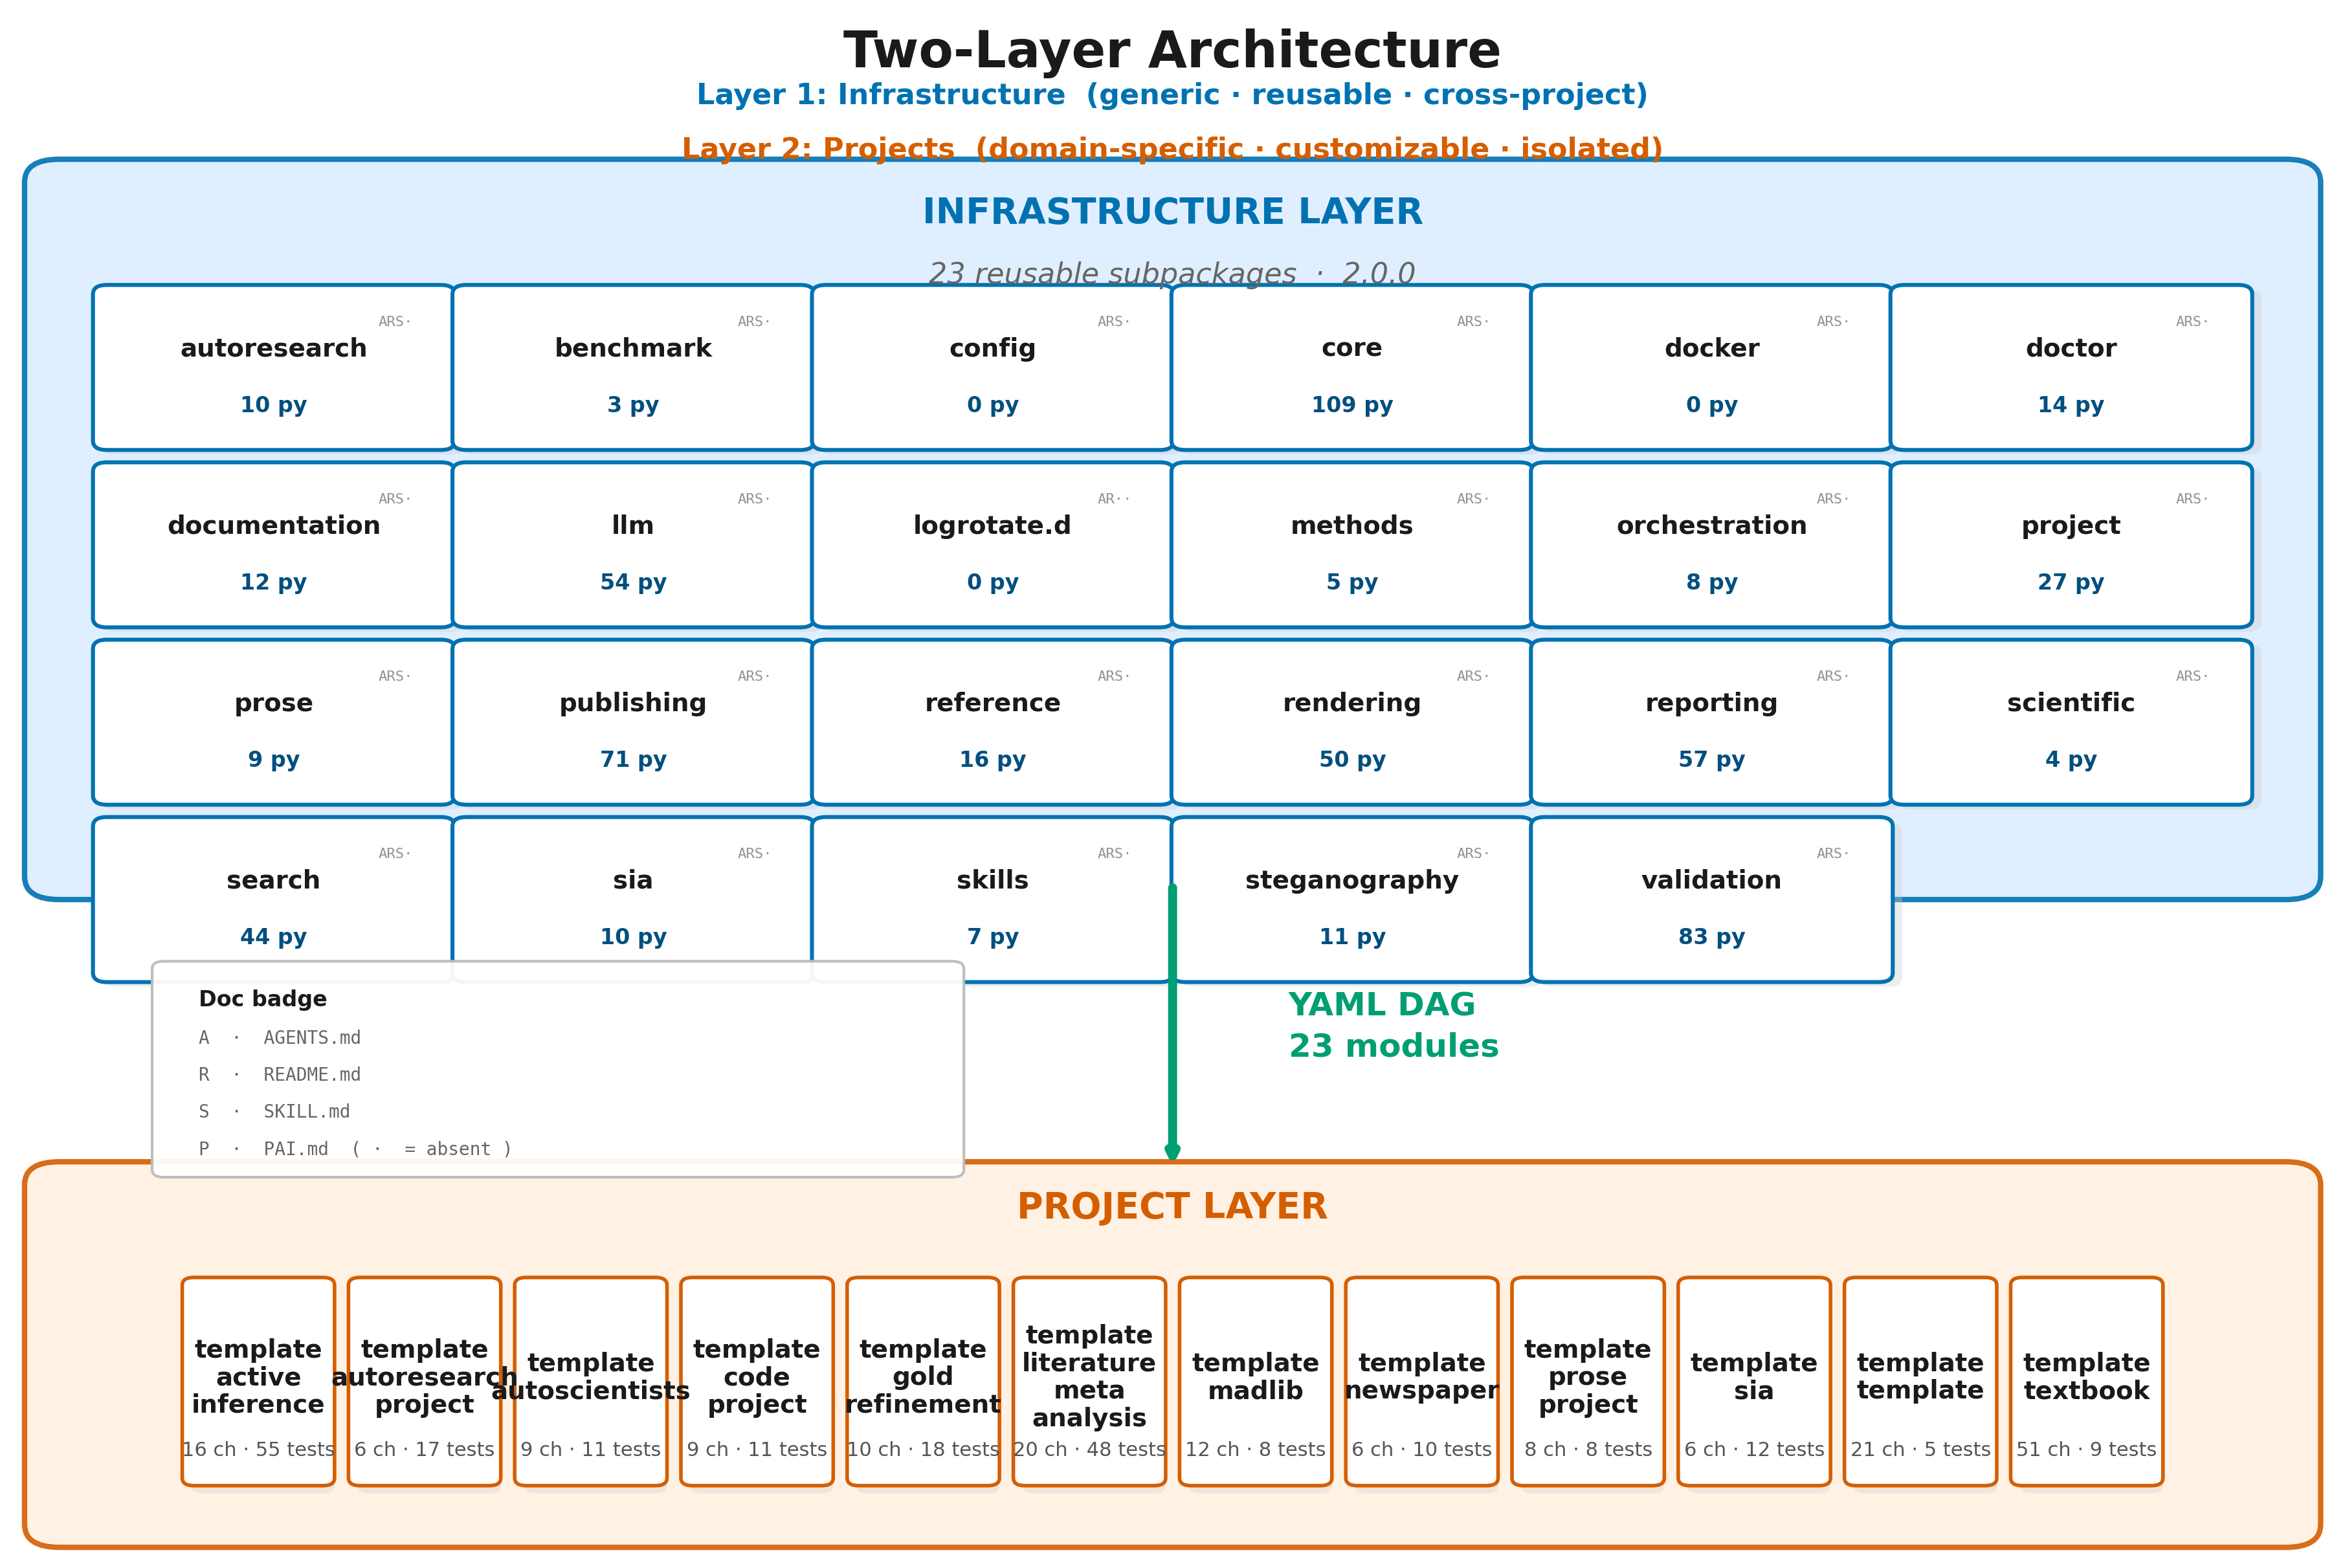
\includegraphics[keepaspectratio,alt={Two-Layer Architecture Overview}]{../figures/architecture_overview.png}}
\textbf{Figure 1.} Live rendering of the Two-Layer Architecture from
repository introspection: the infrastructure layer (top) holds the
\texttt{23} reusable subpackages, each annotated with its Python file
count and a four-slot documentation badge---\texttt{A} AGENTS.md,
\texttt{R} README.md, \texttt{S} SKILL.md, \texttt{P} PAI.md, with
\texttt{·} marking an absent file---so a fully documented module reads
\texttt{{[}ARSP{]}}. A YAML DAG arrow connects it to the project layer
(bottom) of public exemplars labelled with chapter and test counts. The
takeaway: documentation-duality coverage is near-uniform across the
infrastructure, and every box was placed from the same live data the
prose cites.

\pandocbounded{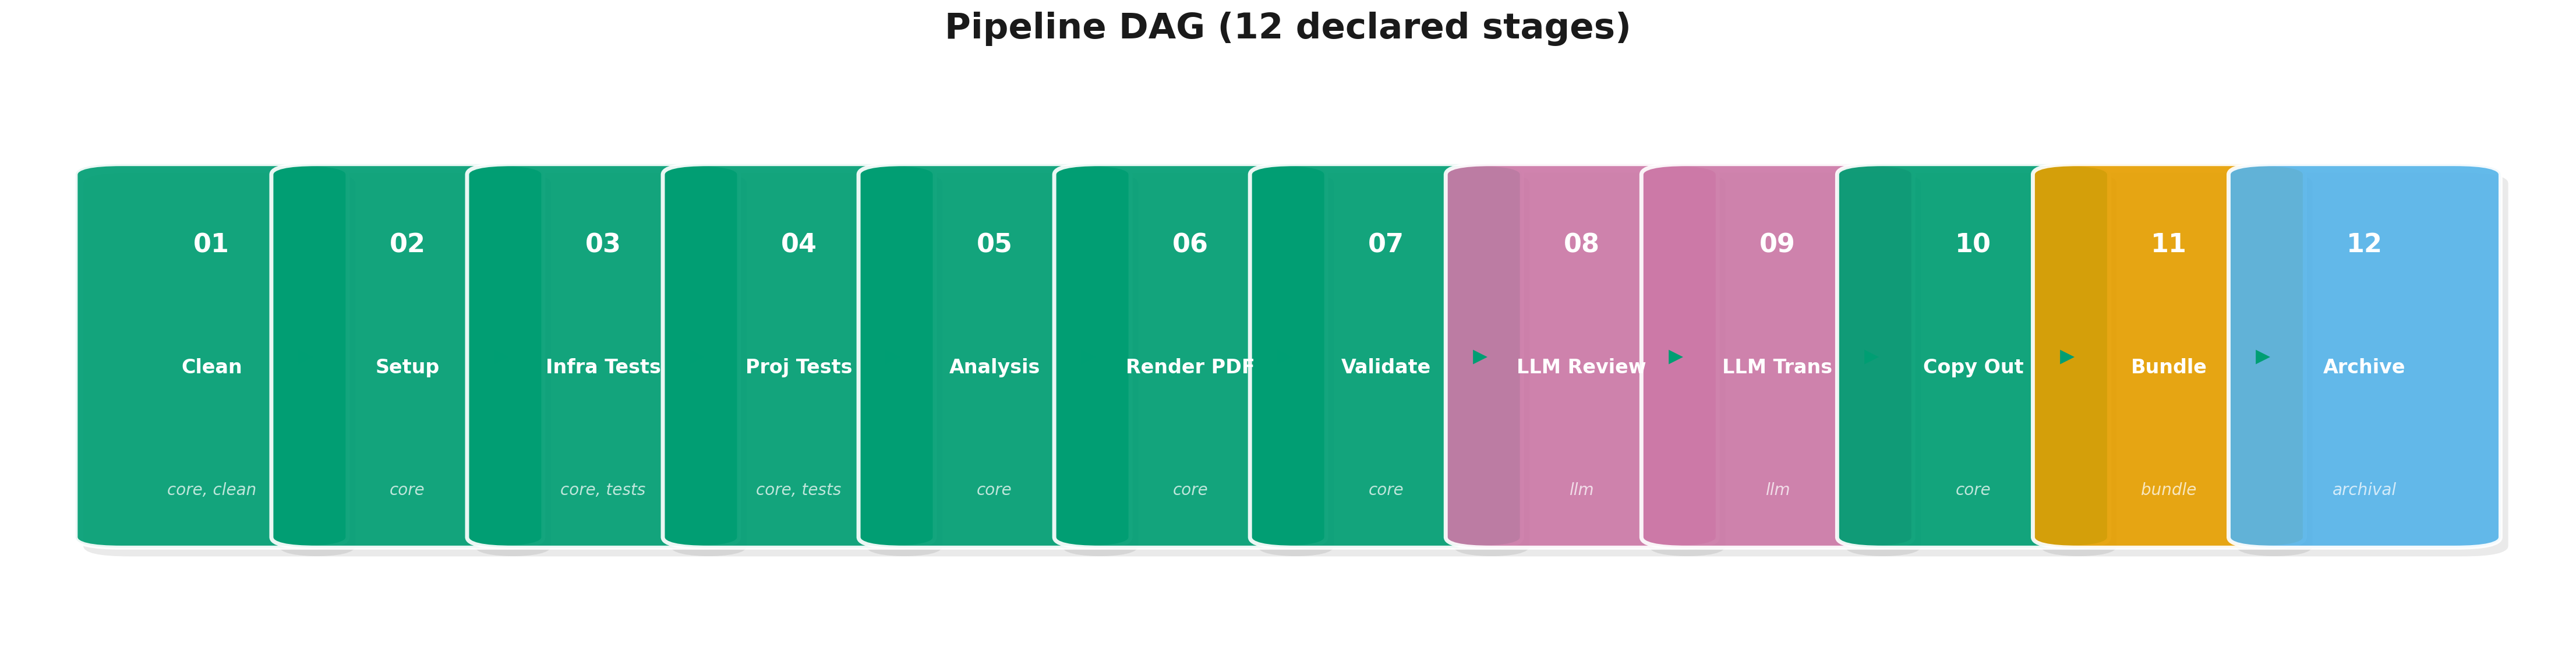
\includegraphics[keepaspectratio,alt={Pipeline Stage Flow}]{../figures/pipeline_stages.png}}
\textbf{Figure 2.} Pipeline DAG with 12 YAML-declared stages (core, LLM,
bundle, archival tags).

\pandocbounded{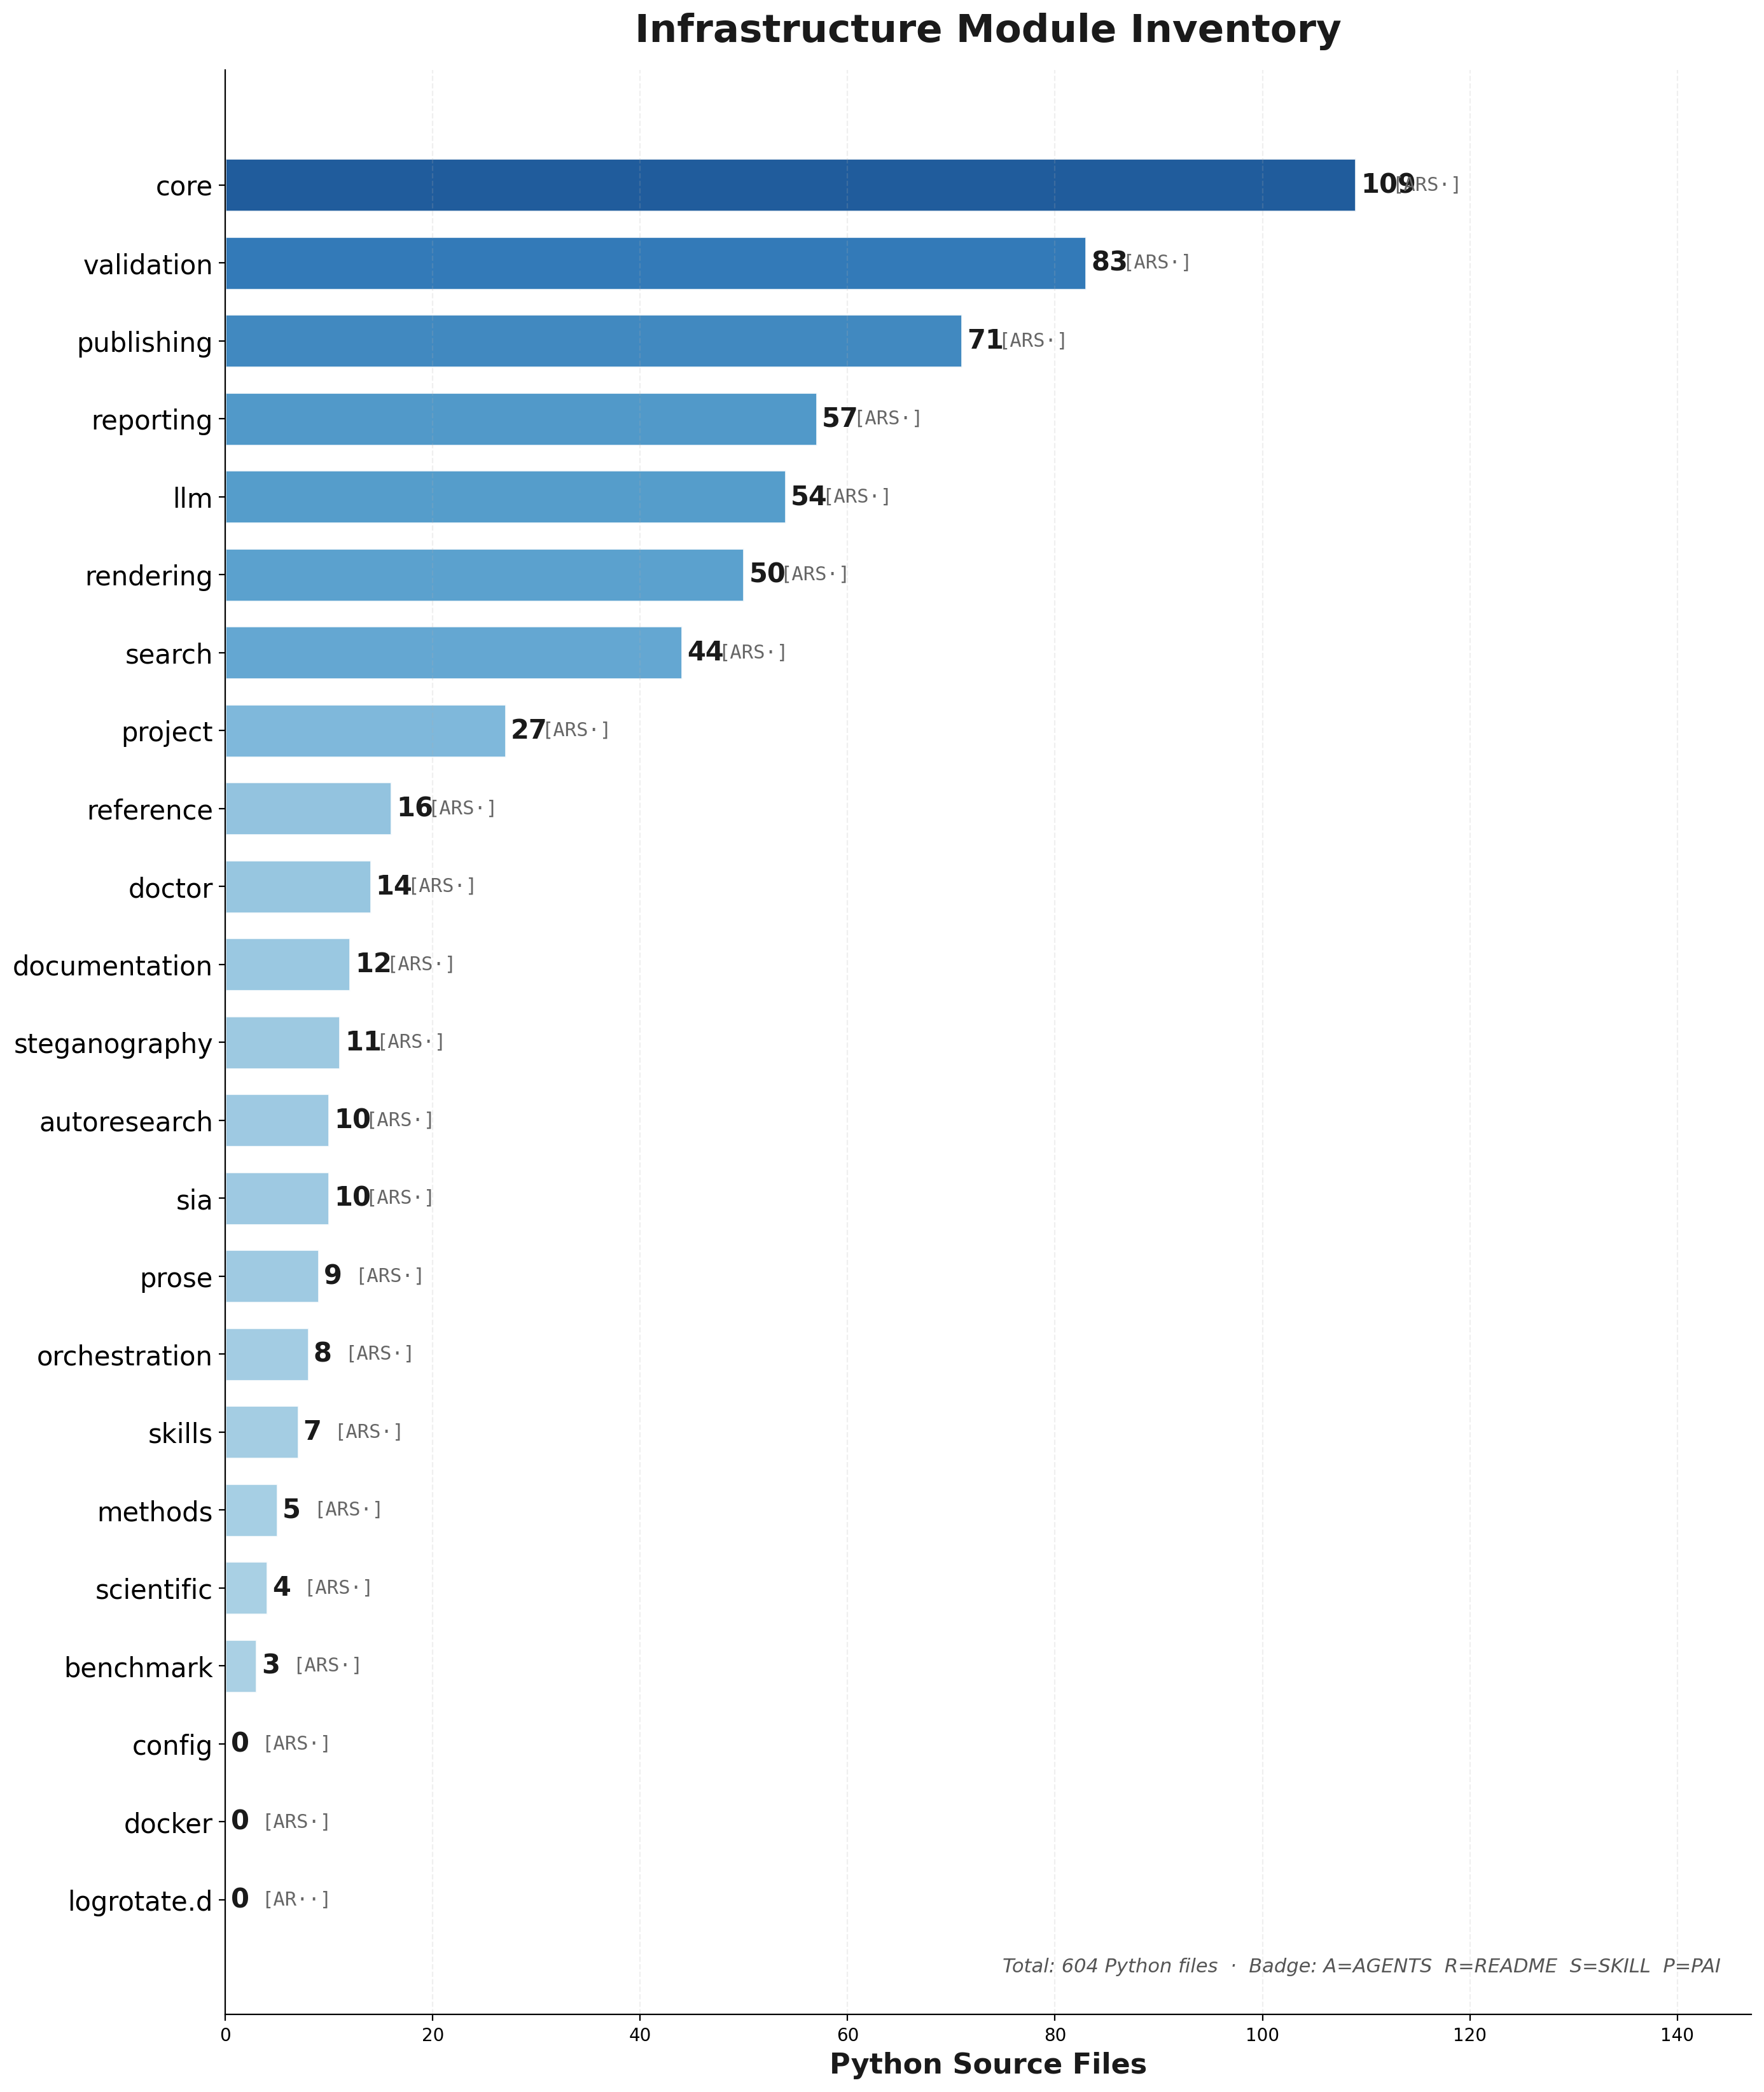
\includegraphics[keepaspectratio,alt={Infrastructure Module Inventory}]{../figures/module_inventory.png}}
\textbf{Figure 3.} Horizontal file-count histogram of every
infrastructure subdirectory, sorted largest-first. The long tail of
small, single-purpose packages beside a handful of larger ones
(\texttt{core}, \texttt{validation}, \texttt{publishing}) is the visual
signature of the Unix-philosophy modularity the architecture section
argues for---capability concentrated where it compounds, not spread
evenly by fiat.
\end{frame}

\begin{frame}[allowframebreaks]{Comparative Feature Analysis}
\protect\phantomsection\label{comparative-feature-analysis}
Figure 4 summarizes the Appendix F capability matrix.

\pandocbounded{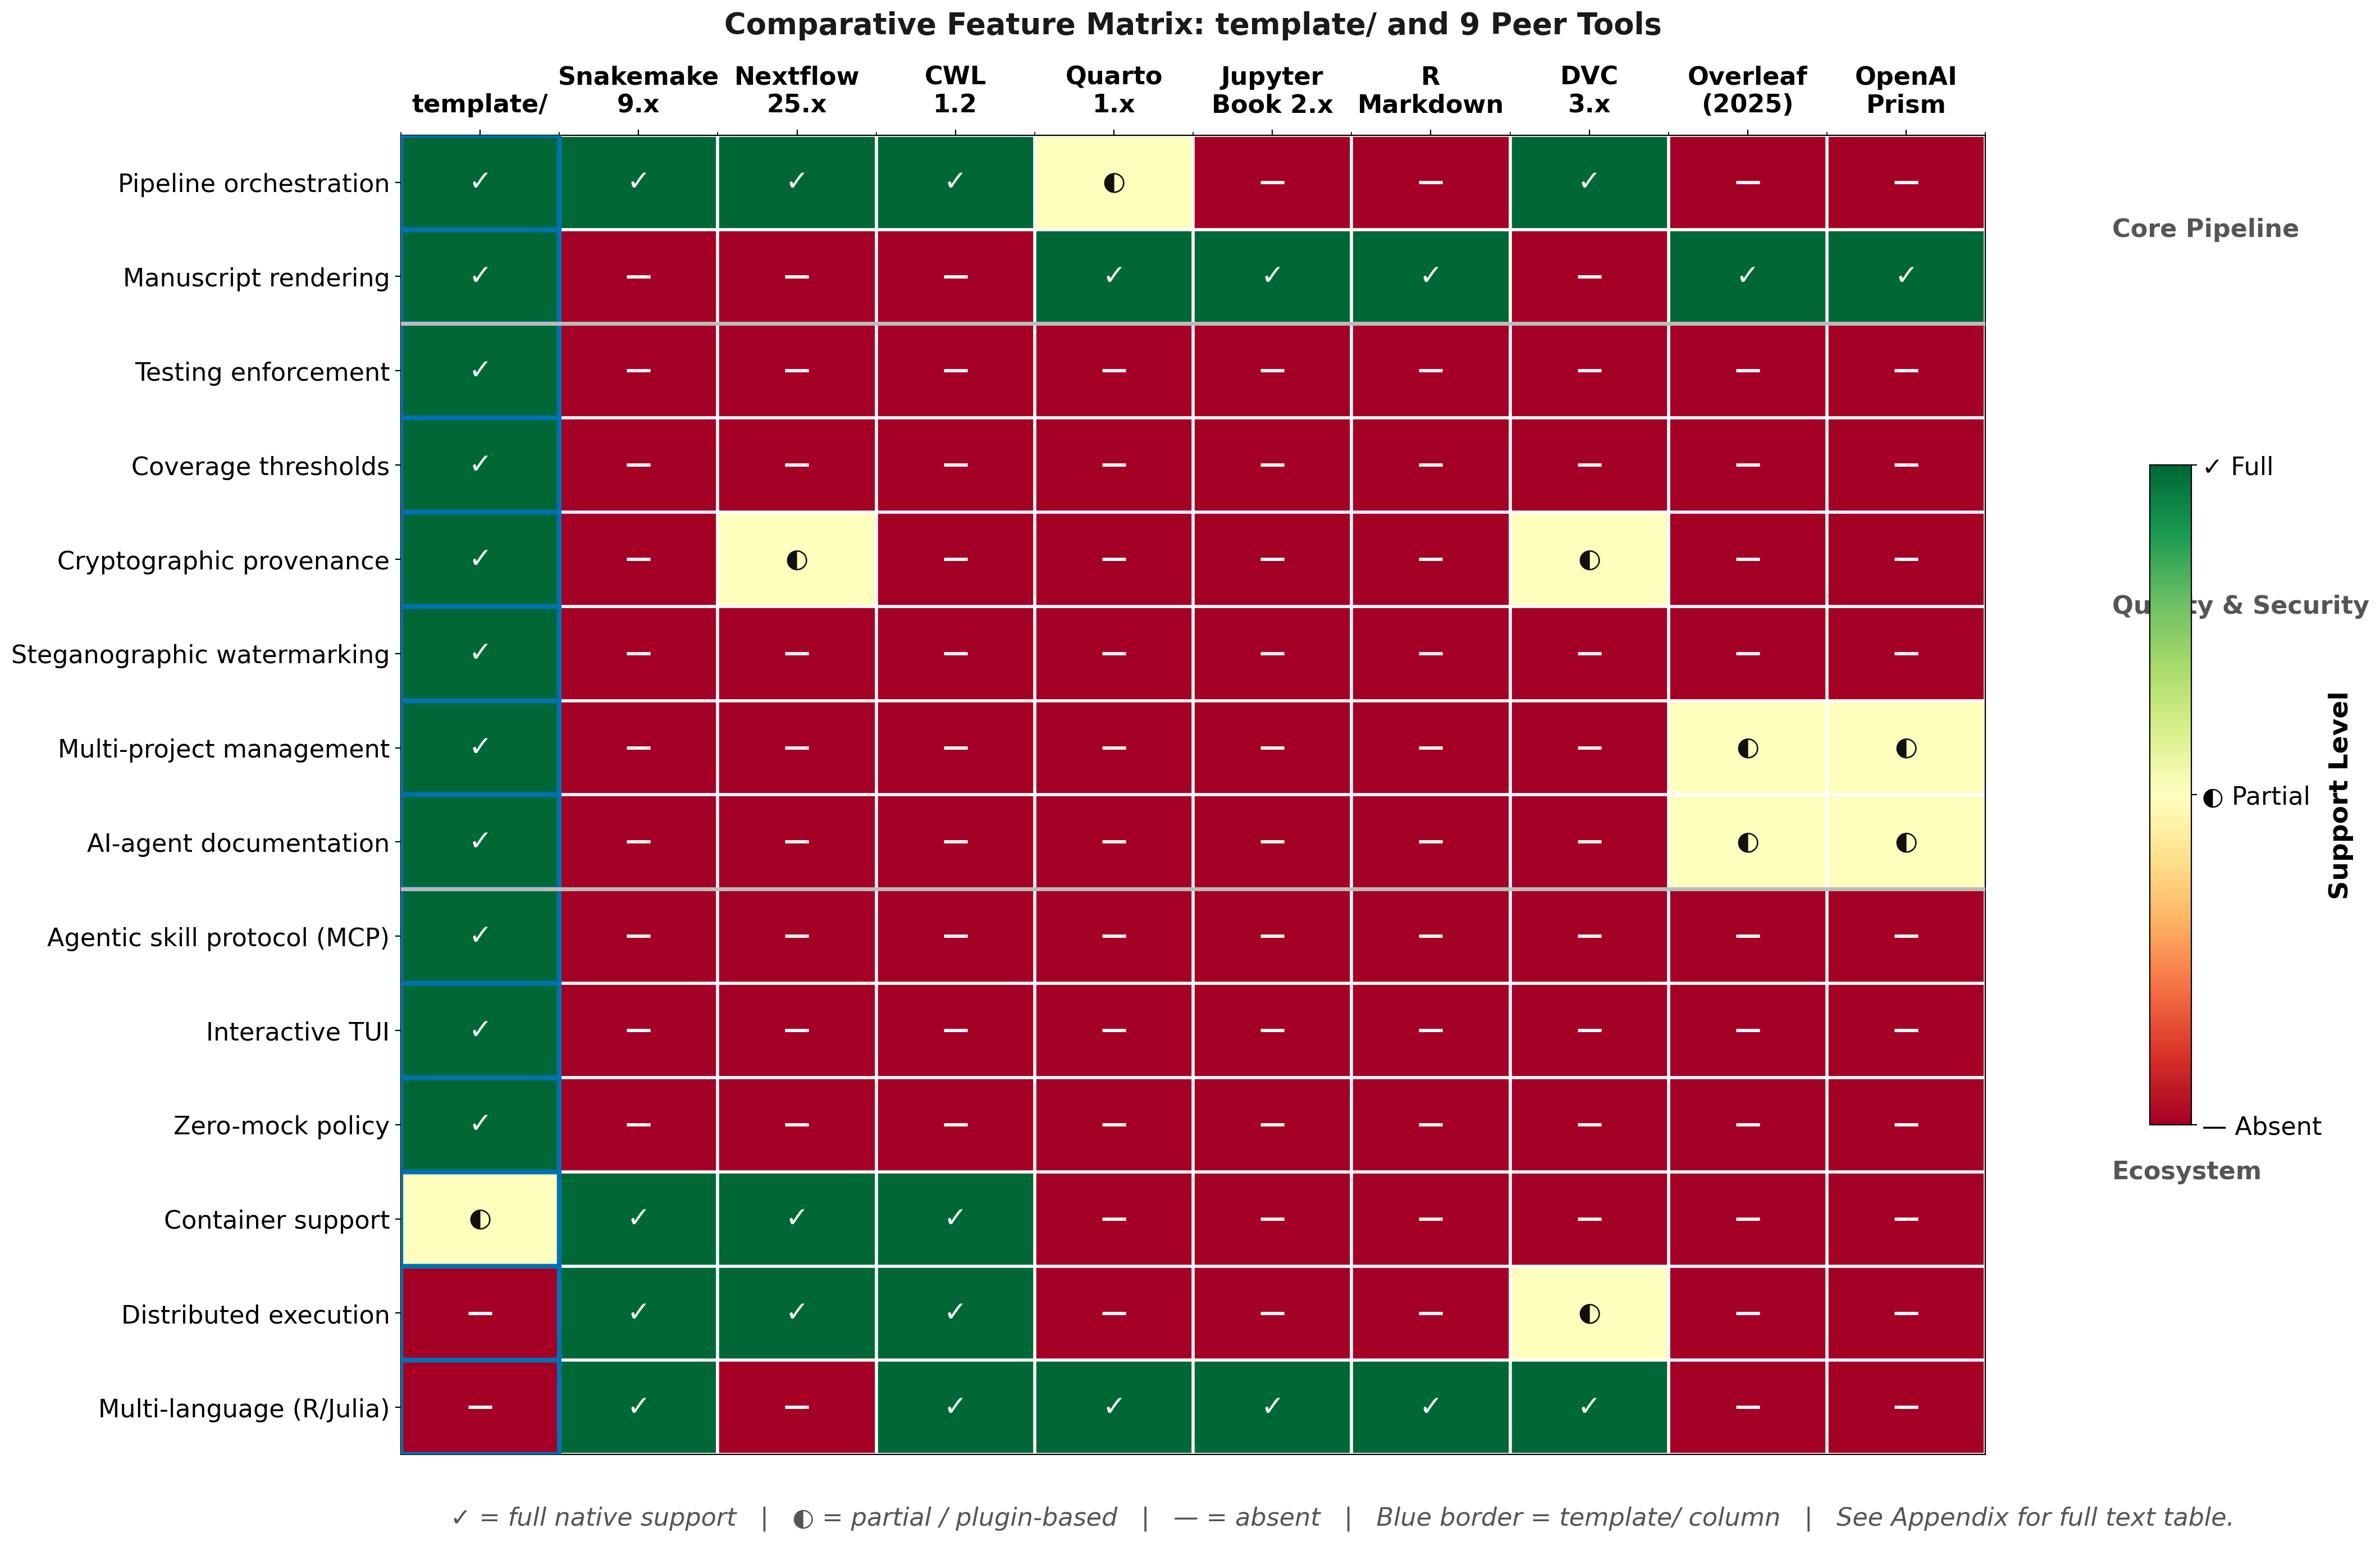
\includegraphics[keepaspectratio,alt={Comparative Feature Analysis Heatmap}]{../figures/comparative_feature_matrix.png}}
\textbf{Figure 4.} 14\,×\,10 heatmap annotated in appendix text---green
\textbf{✓} full native capability, yellow \textbf{◐} partial /
plugin-hosted, red \textbf{---} unavailable. Rows group \emph{Core
Pipeline}, \emph{Quality \& Security}, then \emph{Ecosystem}.

¹ Nextflow 25.04.0: lineage records exist at workflow scope, not per
rendered PDF citation graph.

² DVC: content-addressed artifacts without native prose rendering.

³ DVC: remote object stores (S3, GCS, Azure) without turnkey CI
manuscript gates.
\end{frame}

\begin{frame}[fragile,allowframebreaks]{Test Quality Metrics}
\protect\phantomsection\label{test-quality-metrics}
\begin{itemize}
\item
  \textbf{Zero mocks:} repository policy bans \texttt{unittest.mock} /
  patching frameworks in tests.
\item
  \textbf{Filesystem + subprocess realism:} ephemeral directories +
  actual CLI binaries.
\item
  \textbf{HTTP realism:} infra suites favour \breaktt{pytest-httpserver};
  literature tests hit recorded fixtures.
\item
  \textbf{\breaktt{template\_code\_project}} focuses on numerical
  reproducibility assertions.
\item
  \textbf{\breaktt{template\_autoresearch\_project}} exercises the
  AutoResearch readiness planner
  (\breaktt{infrastructure/autoresearch/}).
  \textbf{\breaktt{template\_search\_project}} exercises
  literature-search workflows.
\end{itemize}
\end{frame}

\end{document}
